\documentclass{article}
\usepackage[a4paper]{geometry}
\usepackage{a4wide}
\usepackage{graphicx}
\title{Boids report}
\author{Joakim Warholm}
\date{March 2019}

\begin{document}
\maketitle
\section{Introduction}
This report describes an implementation of the flock simulator boids, using object-oriented programming (OOP) in python. Some of the principles of OOP used in this implementation are described, and the design choices are discussed.

\section{Technical Background}
\subsection{Inheritance}
When a class inherits attributes and methods from another class it receives those methods and attributes for itself, and becomes a \emph{subclass} of the class it inherits from, while the class it inherits from is called the \emph{superclass} of that subclass \cite[p.60]{PhillipsDusty2010P3oo}. A class called ``car'' might inherit from a class called ``vehicle,'' since a car is a type of vehicle. Then a class called ``volvo'' might inherit from ``car,'' because a vovlo is a type of car. 

\subsection{Static attributes}
A static attribute is an attribute at the class level, meaning it does not belong to one specific object, but rather to one specific class, and all objects of that class share that attribute (meaning that that attribute has the same value for all object of that class). A static attribute can be accessed before an instance of the class that attribute belongs to is made. 

\section{Design}
The boids follow three rules: cohesion, which makes the boids try to flock together; alignment, which makes the boids try to have a common velocity; and separation, which makes the boids try to not crash into each other. The boids have a sight radius, and will only try to flock together when they see each other. The hoiks only follow the separation rule, trying to avoid crashing into other hoiks. Each hoik will try to eat the boid closest to it, no matter how far away that boid is. The boids make no effort to avoid the hoiks. There are two obstacles on the screen, which both hoiks and boids will try to avoid when they get close enough to see it. They will also try to avoid the borders of the screen: when the boids and hoiks get close to a border it will experience an acceleration in the opposite direction. Boids and hoiks can be spawned in by the user. 

\begin{figure}[h!]
    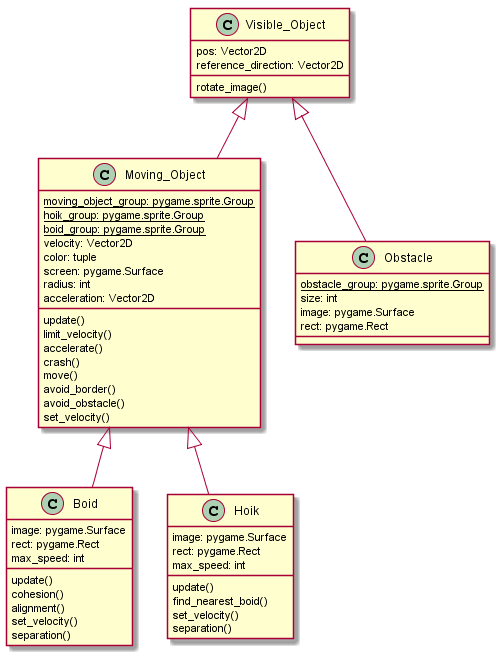
\includegraphics[width = 0.9\textwidth]{Boids.png}
    \caption{UML diagram}
    \label{fig: uml}
\end{figure}

\section{Discussion}
The boids and hoiks are drawn as triangles, while the obstacles are drawn as circles, but their hitboxes are all rectangular, which means things will collide when it looks like they don't. Pixel perfect hit detection is possible by using pygame.mask, but this would lead to a big hit in performence, so it was not used. Another possible solution when it comes to the obstacles would be to use the given \emph{intersect\_rectangle\_circle} function given in the \emph{vector} module, but this would not allow for use of pygame's easily accesible groupcollide method. 

\paragraph{}

The hoiks and the boids have a separation method which is almost identical, the only difference being that boids try to avoid crashing into other boids, while hoiks try to avoid crashing into other hoiks. A much more elegant solution would be to have the separation method in the Moving\_Object class, where it makes the moving object in question try to avoid objects of its own type. At the time of writing that part of the code the solution for how to do that was not found, and so the implementation stayed as it is. 

\section{Conclusion}
This report has described an implementation of the classic flock simulator boids, where OOP principles like inheritance was used. The concepts of inheritance and static attributes have been described, and some of the design choices have been discussed. 

\bibliography{bibl}
\bibliographystyle{plain}

\end{document}